\section{SNR}
\subsection{Définition du SNR}

Le rapport "Signal à bruit" (Signal to Noise Ratio) dans notre cas correspond à :

\[
\text{SNR}_\text{planète}=\frac{\text{Signal}}{\text{Bruit}}=\frac{\text{Nombre de photon de la planète}}{\sqrt{\text{Nombre de photon de l'étoile}}}=\frac{N_\text{planète}}{\sqrt{N_\text{étoile}}}=\frac{N_p}{N_e}
\]

Notre but est donc de \textbf{maximiser} ce rapport, dans le but d'avoir le plus de photon de la planète.

On considère le bruit comme la racine des photons de l'étoile, car on suppose qu'elle suit une loi de Poisson (propriété du bruit de photon).

$\sqrt{N_\text{photon}}=$ fluctuations statistique produit par la lumière "fuyante" de l'étoile (star leakage)

Le bruit de photons, sur une mesure de $N$ photons, est $\sqrt{N}$.



\paragraph{Bruit de photon} Étant donné que les photons de l'étoile sont envoyés aléatoirement, pour un grand nombre de photon la distribution de photon suit une loi gaussienne

En effet, une loi de Poisson de paramètre $\lambda$ correspondant au nombre moyen d'occurrences dans un intervalle de temps fixé, à pour écart type $\sigma = \sqrt{\lambda}$, représentant la dispersion possible des photon de l'étoile dans notre zone de calcul

On peut considérer le SNR comme un intervalle de confiance $\sigma$ de la qualité de notre mesure. Ainsi, pour pouvoir confirmer la détection d'une exoplanète, il faut au minimum 

\[
\text{SNR}\geq 5
\]

\subsection{Calcul du SNR}


Ainsi, à partir d'une PSF obtenue, nous souhaitons calculer le SNR de l'apodiseur.
Sur notre PSF, nous n'avons que l'image de l'étoile diffracté à travers la pupille de l'ELT. Pour réaliser ce calcul, nous procédons ainsi : comme l'image ne simule que l'image de l'étoile (et ne comprends pas les pixels d'une potentielle exoplanète), nous allons calculer le nombre de photon de la planète $N_p$ tel qui suit : 
\paragraph{$N_p$}
Sur l'image, on somme la valeur de chaque pixel (correspondant à l'intensité lumineuse) compris à l'intérieur du coeur de l'étoile (aussi coeur de la PSF), qu'on va ensuite diviser par le nombre de pixel à l'intérieur du cercle pour obtenir une intensité moyenne (correspond à \texttt{intensite\_coeur\_PSF}). Ensuite, comme on considère que la planète est $10^{-7}$ fois moins lumineuse que l'étoile, on multiplie l'intensité par ce facteur.

\quad - On calcule bien l'\textbf{intensité} et non le \textbf{contraste} dans la zone (meme si en vrai ça donne le même rapport donc on s'en fout ? mais physiquement c'est débile un peu du coup)

Ensuite, afin de connaître le nombre de photons lié à cette zone, on utilise une fonction \texttt{PhotonCount} qui calcule la quantité de photon collecté par un télescope en fonction du temps d'exposition, des paramètres de longueur d'onde d'observation et la surface du telescope. Ainsi, cela correspondra environ à l'entièreté des photons compris dans la PSF.
Pour trouver le nombre de photon dans la zone, il suffit de faire une règle de 3 en divisant le tout par intensite totale de la PSF, donc en moyenant tous les pixels composant la PSF
\paragraph{$N_e$}
De même, pour connaitre le nombre de photons de l'étoile $N_e$, on réalise une règle de 3 similaire, sauf que l'on compte l'intensité totale dans la zone où on estime que le coeur de la planète se trouvera (que l'on calcule avec la fonction \texttt{intensite\_in\_Sp}), puis on multiplie par le nombre de 

On peut résumer cela par les équations :
\begin{align*}
    \boxed{N_p = \gamma \times \frac{I_{\in\: S_e}}{I_{tot}} \times  C} \qquad \boxed{N_e = \gamma \times \frac{I_{\in \:S_p}}{I_{tot}}}
\end{align*}

avec $\gamma$ le nombre de photons total dans la PSF, $C$ le contraste considéré pour la planète, $I_{tot}$ l'intensité totale dans la PSF

\begin{figure}[htbp]
    \centering
    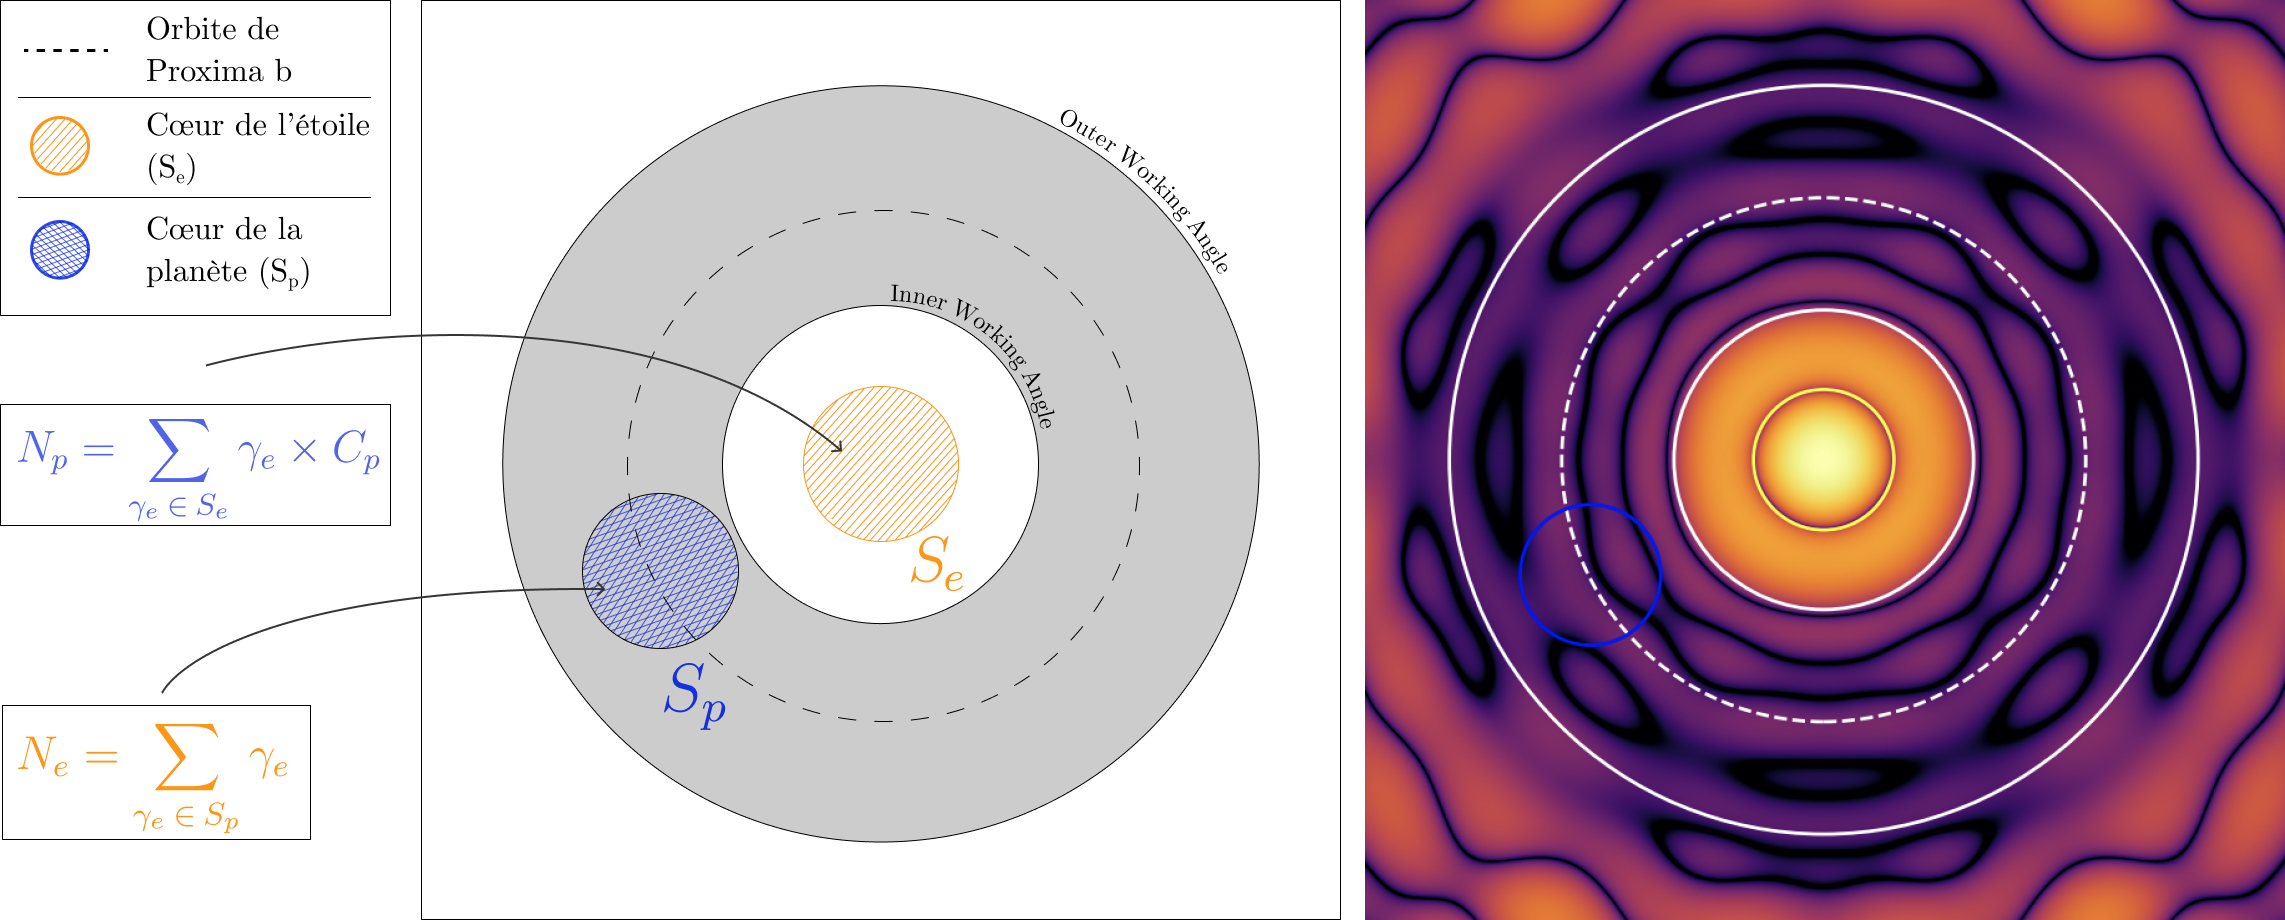
\includegraphics[width=\textwidth]{figures/v2_expl_snr.png}
    \caption{Représentation des différents éléments permettant le calcul du SNR. À droite, on représente les zones considéré dans une PSF créer par un apodiseur de paramètre 2.6 6.5 0.69}
\end{figure}


Ainsi, ce calcul nous donne le SNR pour un apodiseur donnée, mais également pour le cas de la pupille seule de l'ELT.

En effet, le but final d'un apodiseur est de permettre une meilleur observation de la planète, et doit donc avoir un meilleur SNR que s'il n'y en avait pas. 

Pour calculer ça, on va alors comparer le SNR d'un apodiseur par rapport à celui de la pupille en absence d'apodiseur, et vérifier que ce nombre est bien supérieur à 1

\subsection{Calcul du rapport de SNR : SNR\%}

Notre but va être alors de maximiser ce rapport. En effet, on peut considérer que notre gain de temps de telescope correspond au carré de ce rapport. Pour un gain de SNR de 3, le temps de telescope est divisé par 9, permettant ainsi plus d'observation pour un prix moins élevé.

Pour calculer ce rapport, il suffit de calculer le SNR de la pupille avec les mêmes paramètres qui ont été choisi pour calculer le SNR de la PFS de l'apodiseur tel que 

Il ne faut pas oublier qu'un apodiseur implique forcément un facteur de transmission, car elle bloquera toujours plus de lumière que la pupille seule. Pour calculer la transmission d'un apodiseur, on calcule le rapport de la surface de la pupille de l'ELT comparé à la surface de l'apodiseur, qui sera forcément plus grande.

\[\text{SNR\%}=\frac{\text{SNR}_\text{apod}}{\text{SNR}_\text{pup}}=\dfrac{\dfrac{N_p\times t}{\sqrt{N_e\times t}}}{\dfrac{N_p}{\sqrt{N_e}}}\]

\subsection{Variation du gain de SNR en fonction de la transmission (IWA, OWA fixés)}

Expliaction du princiep

Faire différents exemple pour montrer ? jsp 

Ce qu'on peut conclure par rapport à la transmission 

Mention de l'apodiseur gris à ce moment là ? 

\subsubsection{Impact de l'optique adaptative — Première approximation}

On va maintenant considérer le flou créer par le mouvement des accuateurs / miroirs qui vont venir empecher d'atteindre le vrai contraste atteignable par l'apodiseur.

SCHEMA

\subsection{Recherche du meilleur apodiseur}

Chercher le meilleur apodiseur revient à chercher quels paramètres obtiennet le meilleur gain en SNR.

Avant de chercher cette apodiseur, nous devons déjà considérer les contraintes imposé par la situation pour limiter notre espace de paramètres.

On pose ainsi nos conditions :

\begin{itemize}[label=\textendash]
    \item La planète doit être visible dans toute la dark zone dans toute la bande H
        \begin{itemize}
            \item c-a-d que les owa sont assez grand pour observer proxima b à la plus petite longueur d’onde de la bande H (1.4 µ), soit quand l’owa est le plus petit
            \item les iwa sont assez petits pour observer proxima b à la plus grande longueur d’onde (1.8 µ), soit quand l’iwa est le plus grand
        \end{itemize}
    \item On veut également que la zone commune entre l’owa$(\lambda _{min})$ et l’iwa$(\lambda_{max})$ fasse au moins la taille du coeur de l’étoile à $\lambda _{max}$, soit $2.44\: \lambda_{max}/D$. Cela permet de s’assurer que l’on peut bien récupérer toute les informations de la planète dans toute la bande H et que lorsque qu’on fait une observation moyenné, qu’on ait bien une zone où toute l'information de la planète est présente
\end{itemize}

Nous avons imposé un IWA minimum de 2.0 et un OWA maximum de 7.0, afin de ne pas être trop proche de l’étoile ni d’avoir une dark zone trop grande empechant de trouver un résultats suffisant possible 

% On peut voir que les dark zone débutant à 2.0 $\lambda /D$ ont généralement un gain trop faible

\begin{figure}
    \centering
    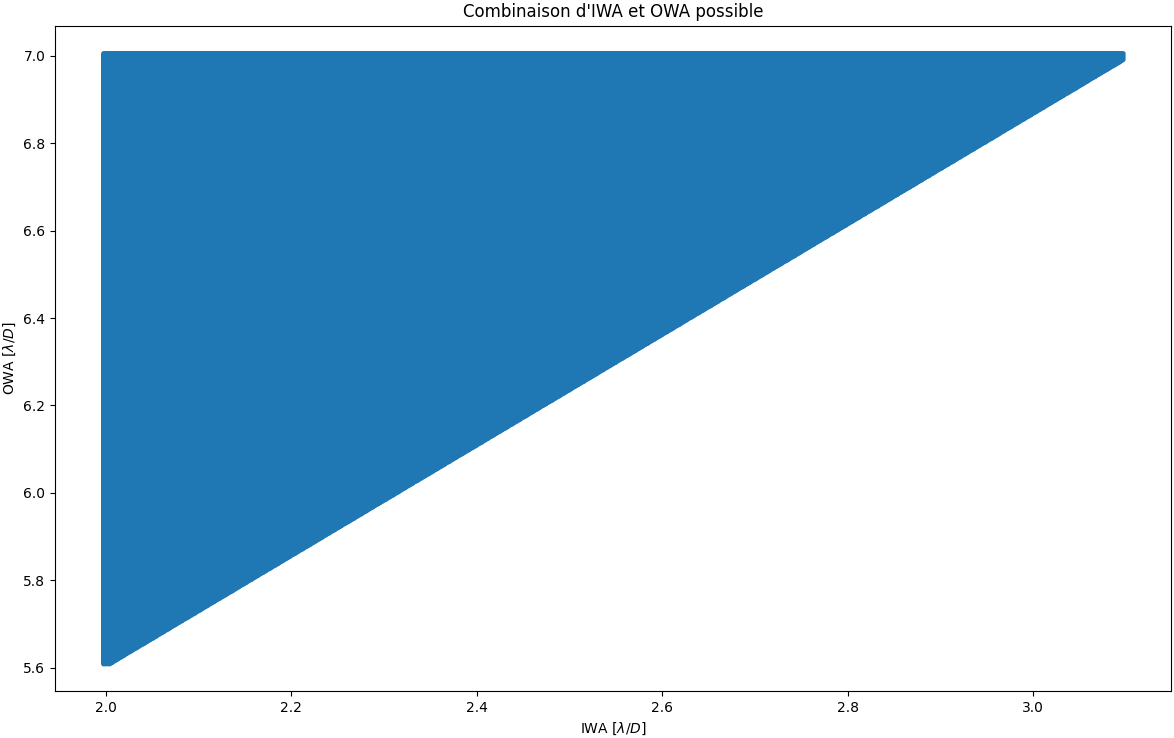
\includegraphics[width=0.6\textwidth]{figures/comb_iwa_owa_hq.png}
    \caption{test}
\end{figure}
%euh va clairement falloir refaire le graphique avec des axes plus grands omg

Ainsi, en limitant notre espace, nous obtenons que les OWA vont de 5.62 à 7.00 et les iwa de 2.00 à 3.09. 
En arrondissant, nous considérerons donc notre espace de paramètres comme

\[
\begin{cases}
\text{IWA} \in [2.00 - 3.00] \\
\text{OWA} \in [5.75 - 7.00]
\end{cases}\]



% \begin{lstlisting}[language=Python]

%     def EnerEncercl(image, nombr_pix, diam_coeur):
%     """
%     Permet de calculer le contraste moyen dans le coeur de l'etoile (moy_coeur) et dans le champ de vue (moy_FOV)

%     Parameters:
%         image (NDArray) : Array correspondant a la matrice de contraste de la PSF [1024 x 1024]
%         nombr_pix (int) : entier correspondant a la largeur de l'image en pixel (minim 2*fov pour respecter la limite de Shannon)
%         diam_coeur (float) : correspond a la largeur totale (soit au diametre) du coeur de la PSF, soit (2.44 L/D) converti en pixels
    
%     Returns:
%         tuple : moy_FOV, moy_coeur
%     """
%     # Creer un tableau d'indices pour les coordonnees
%     y, x = np.indices((nombr_pix, nombr_pix))
    
%     # Calculer la distance de chaque point par rapport au centre
%     center = nombr_pix / 2
%     distances = np.sqrt((x - center)**2 + (y - center)**2)
    
%     # Creer un masque pour les pixels a l'interieur du coeur de la PSF
%     coeur_mask = distances <= diam_coeur / 2
%     coeur_throughput = distances <= (diam_coeur / 2.44 * 1.5) / 2
    
%     # Calculer les sommes
%     moy_FOV = np.mean(image)
%     moy_coeur = np.mean(image[coeur_mask])
%     moy_through = np.mean(image[coeur_throughput])

%     return moy_FOV, moy_coeur, moy_through


%     def PhotonCount(T, S, lambda_0, BW, mag, mag_type, throughput, WORKPATH='/Users/boyerlal/Desktop/'):
%     """
%     T:          exposure time [s]
%     S:          telescope surface [m2]
%     lambda_0:   central wavelength [nm]
%     BW:         bandwidth [nm]
%     mag:        apparent magnitude of the star
%     mag_type:   magnitude system: either 'AB' or 'VEGA'
%     throughput: telescope+instrument throughput. It does not include the coronagraph throughput.
%     """
%     if platform.system() == 'Darwin':
%         WORKPATH = '/Users/lalyboyer/Desktop/'
%     if mag_type == 'AB':
%         AB_mag = mag
%     elif mag_type == 'VEGA':
%         AB_mag = mag + AB2V_CONVFACT(lambda_0, BW, WORKPATH)
%     else:
%         AB_mag = mag
%         print('Error! Choose between AB mag or VEGA. Switching to AB mag')
%     PC = T * S * throughput * 1.51 * 1e26 / (1e-9 * lambda_0 * 10) * 10**(-(AB_mag + 48.6) / 2.5) * BW * 1e-9 * 10 * 10000
%     return PC

%     contrast_coeur_PSF = EnerEncercl(image, nbr_pix, diam_coeur_pix)[1]
%     contrast_coeur_Pupil = EnerEncercl(PupilIm, nbr_pix, diam_coeur_pix)[1]
%     contrast_tot_PSF = EnerEncercl(image, nbr_pix, diam_coeur_pix)[0]
%     contrast_tot_Pupil = EnerEncercl(PupilIm, nbr_pix, diam_coeur_pix)[0]

%    N_planete = PhotonCount(3600, 978, lamb_0_nm, BW, 4.835, 'VEGA', 0.3) 
%    * (1e-7) * contrast_coeur_PSF / contrast_tot_PSF
%     N_etoile = PhotonCount(3600, 978, lamb_0_nm, BW, 4.835, 'VEGA', 0.3) 
%     * Contrast_in_S(image, nbr_pix, iwa * nbr_pix / fov, owa * nbr_pix / fov, diam_coeur_pix) / contrast_tot_PSF

% \end{lstlisting}


\begin{itemize}[label=\textendash]
    \item pas oublier l’erreur que j’ai fait un moment de pas considérer correctement le SNR\% maximum (que plus c’est flou plus faut augmenter la transmission pour compenser)
    \item tentative de cherecher la combi d’apod pour harmoni, ça a pas abouti :/
    \item bcp de temps passer a vouloir optimiser le calcul de SNR\%
    \item juste les calculs finaux pour voir qu’est ce qui rend le meilleur SNR\%
    \item sachant que j’ai du faire des bidouilles obscures pour afficher correctemnet, pas oublier ça
\end{itemize}

\subsection{Interprétation de sa valeur ($>$5 pour SNR, $>$1 pour le SNR\%)}

\subsection{L’impact de l’OA sur les PSF vu par les valeurs de SNR associées}

\subsection{Dichotomie pour déterminer les meilleurs paramètres d’apodiseur}